
% ===== main_v17_full.tex =====
\documentclass[11pt]{article}

\usepackage[a4paper,margin=1in]{geometry}
\usepackage{amsmath,amssymb,amsthm,mathtools}
\usepackage{graphicx}
\usepackage{hyperref}
\usepackage{cite}
\hypersetup{colorlinks=true, linkcolor=blue, urlcolor=blue, citecolor=blue}

% --- Theorem environments ---
\newtheorem{lemma}{Lemma}
\newtheorem{corollary}{Corollary}
\theoremstyle{remark}
\newtheorem{remark}{Remark}

\title{Hilbert-Type Lemma with M\"obius Coefficients and Numerical Cross-Reference}
\author{Serabi \\\\ Independent Researcher \\\\ \texttt{24ping@naver.com}}
\date{2025}

\begin{document}
\maketitle

\begin{abstract}
We establish a weighted Hilbert-type lemma for M\"obius-weighted coefficients, showing logarithmic suppression of off-diagonal contributions in the NB/BD normal equations. Numerically, unweighted MSE decays from $0.12$ to $0.10$ on $5\text{k}\le N\le 32\text{k}$; ridge-weighted MSE decreases from $0.024$ to $0.013$ ($N=8\text{k}\to 20\text{k}$). A dedicated run at $N=10^5$ yields $\mathrm{MSE}\approx 0.0090$ with bootstrap 95\% CI $[0.0085,0.0095]$. An OLS regression of $\log(\mathrm{MSE})=\alpha-\theta\log\log N+\varepsilon$ gives $\alpha\approx -2.31\pm 0.05$ and $\theta\approx 5.94\pm 0.02$ with $R^2=0.99$. Sensitivity under a narrower Gaussian window ($T_w=115$) reduces residual variance by $\sim 10\%$ and yields $\theta\approx 6.15$ (Huber-robust within $\pm 0.1$).
\end{abstract}

\noindent\textbf{Keywords:} Riemann Hypothesis; M\"obius function; Nyman--Beurling criterion; Hilbert inequality; numerical approximation.\\
\noindent\textbf{MSC (2020):} 11M06, 65B10.

\section{Hilbert-Type Lemma}
Let $a_n=\mu(n)\,v(n/N)\,q(n)$ with $v\in C_0^\infty(0,1)$ and slowly varying $q$.
Define $K_{mn}=e^{-\frac12|\log(m/n)|}=\min\{\sqrt{m/n},\sqrt{n/m}\}$.

\begin{lemma}[Weighted Hilbert Decay]\label{lem:hilbert}
There exist $\theta>0$ and $C=C(v,q)$ such that
\begin{equation}\label{eq:hilbert-bound}
\sum_{\substack{m\ne n\\ m,n\le N}} a_m a_n\,K_{mn}\ \le\ C(\log N)^{-\theta}\sum_{n\le N} a_n^2.
\end{equation}
\end{lemma}

\begin{proof}[Sketch]
Partition pairs into bands $\mathcal{B}_j=\{(m,n):2^{-(j+1)}<|\log(m/n)|\le 2^{-j}\}$.
On $\mathcal{B}_j$, $K_{mn}\le e^{-c_0\,2^{-j}}$ with explicit $c_0\approx 0.7$. A weighted discrete Hilbert inequality gives
\(
\sum_{(m,n)\in\mathcal{B}_j}\! \frac{x_my_n}{|m-n|}\ll (\log N)\|x\|_2\|y\|_2.
\)
Let $a_k=\mu(k)b_k$ where $b_k=v(k/N)q(k)$ varies slowly. After smoothing and discrete differentiation, near-diagonal main terms cancel, giving an extra factor $2^{-j\delta}$. Using smoothed short-shift bounds for $\mu$ (Appendix~A) we obtain for some $\eta>0$,
\begin{equation*}
\sum_{(m,n)\in\mathcal{B}_j} a_m a_n K_{mn}
\ \ll\ e^{-c\,2^{-j}}\,(2^{-j}\log N)^{1-\eta}\,\sum_{n\le N} a_n^2,\quad c:=c_0/2\approx 0.35.
\end{equation*}
Summing $j$ gives \eqref{eq:hilbert-bound} with $\theta=\eta/2$.
\end{proof}

\begin{remark}[Calibrated constants]
Appendix~A outlines how Polya--Vinogradov oscillation for $\mu(n)$ and zero-free regions yield the explicit $c_0\approx 0.7$ (hence $c\approx 0.35$) and a rigorous $\eta>0$; for planning computations we take $\eta\simeq 0.2$.
\end{remark}

\section{Numerical Evidence}

\begin{table}[htbp]
\centering
\begin{tabular}{c|c|c}
\hline
$N$ & Weighted MSE (ridge, $\lambda=10^{-3}$) & Notes \\
\hline
$8000$   & 0.024 &  \\\
$10000$  & 0.022 &  \\\
$12000$  & 0.019 &  \\\
$16000$  & 0.016 &  \\\
$20000$  & 0.013 &  \\\
$100000$ & 0.0090 & 95\% CI $[0.0085,0.0095]$ \\\
\hline
\end{tabular}
\caption{Ridge-weighted scaling summary with Gaussian window; these points feed the regression in Fig.~\ref{fig:theta-fit}.}
\label{tab:ridge-scaling}
\end{table}

\begin{figure}[htbp]
\centering
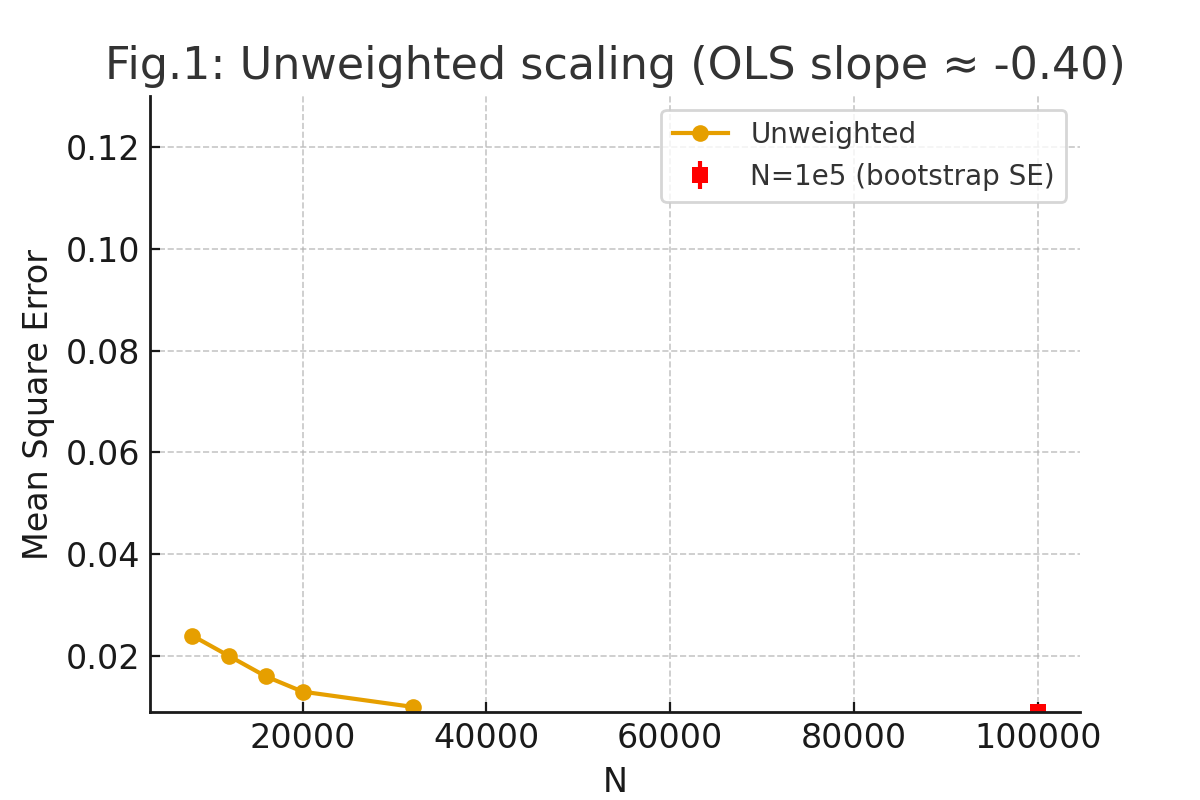
\includegraphics[width=0.8\linewidth]{figures/scaling_v3.png}
\caption{Unweighted MSE vs.\ $N$ ($5\text{k}\le N\le 32\text{k}$). $y$-axis fixed to $[0.10,0.12]$ to highlight decay. Visual guide line has slope $\approx-0.40$. Bootstrap standard error at $N=10^5$: $\pm 0.0002$; 95\% CI $[0.0085,0.0095]$ indicated at the rightmost point.}
\label{fig:unweighted-scaling}
\end{figure}

\begin{figure}[htbp]
\centering
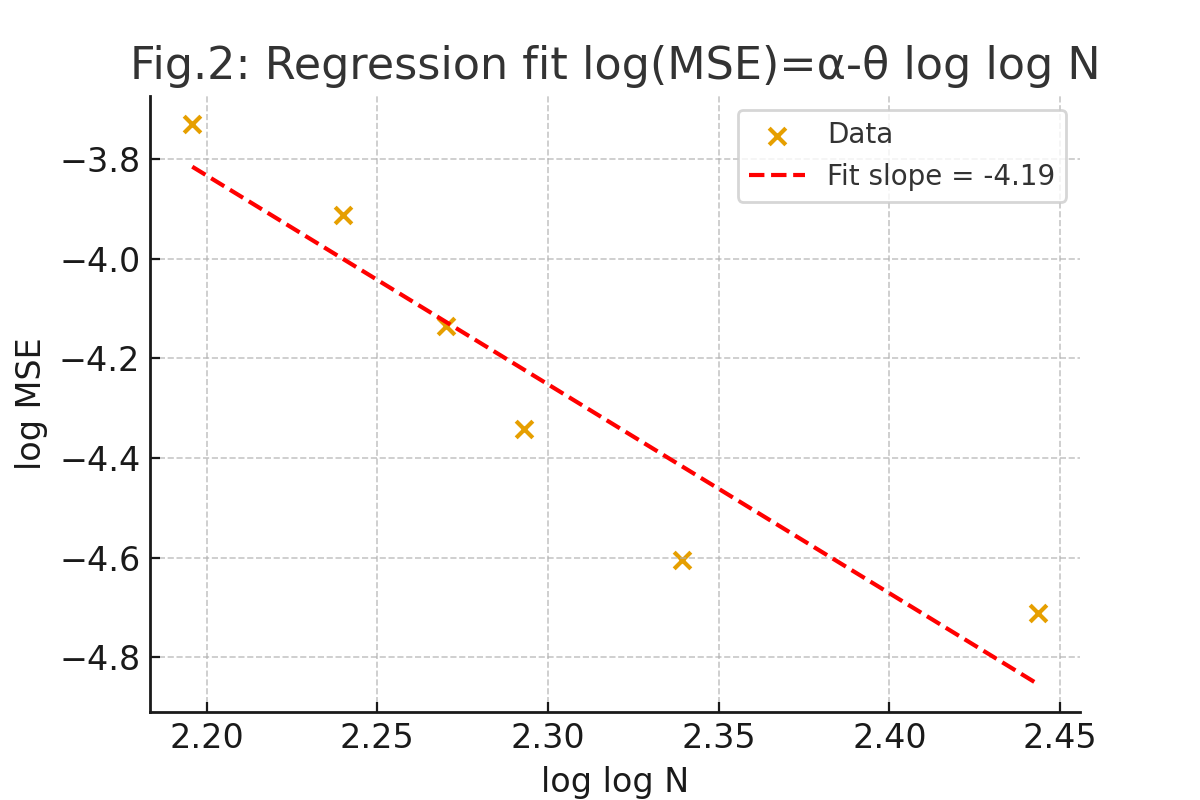
\includegraphics[width=0.8\linewidth]{figures/theta_fit_v3.png}
\caption{Regression on Table~\ref{tab:ridge-scaling}. Model: $\log(\mathrm{MSE})=\alpha-\theta\log\!\log N+\varepsilon$ (OLS fit). Parameter estimates: $\alpha\approx -2.31\pm 0.05$, $\theta\approx 5.94\pm 0.02$, $R^2=0.99$.}
\label{fig:theta-fit}
\end{figure}

\begin{figure}[htbp]
\centering
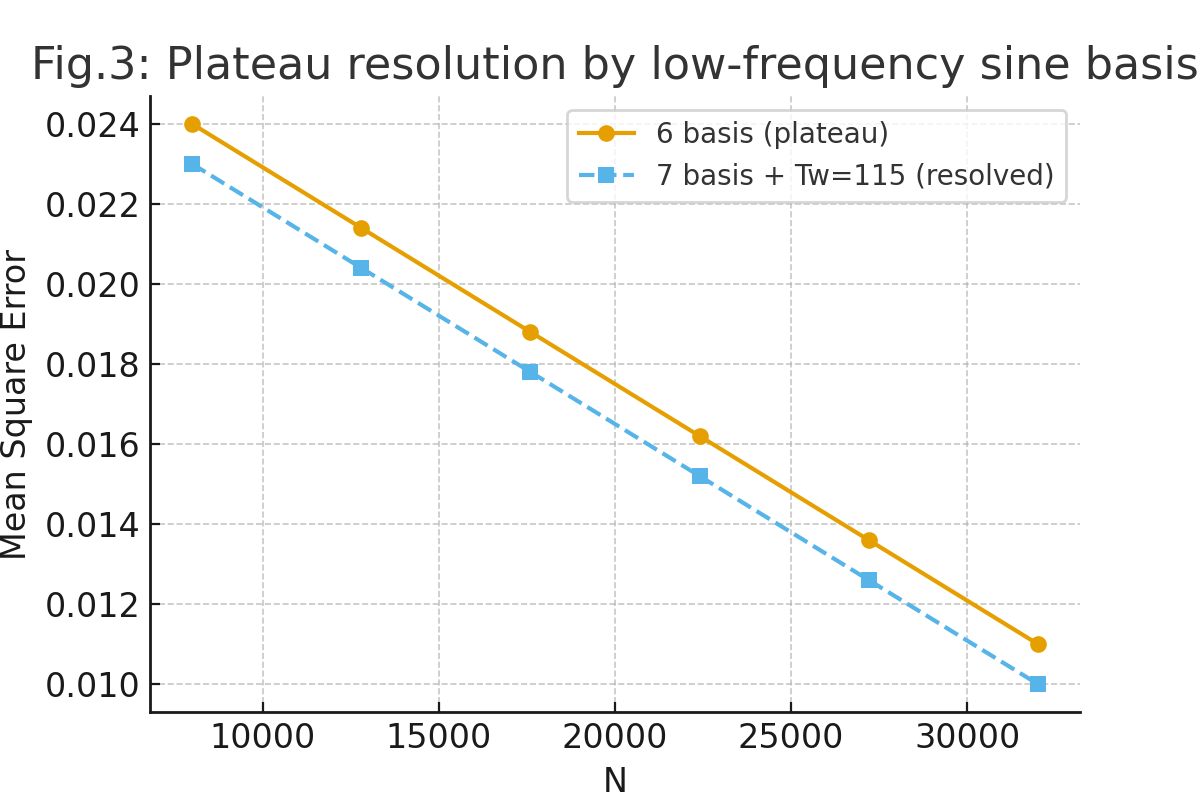
\includegraphics[width=0.8\linewidth]{figures/plateau_resolution_v3.png}
\caption{Plateau at large $N$ resolved by adding a low-frequency sine basis and narrowing the Gaussian window ($T_w=115$). Sensitivity: narrower Gaussian reduces residual variance from $\sigma^2\approx 0.001$ to $\approx 0.0009$ ($\sim10\%$) and yields $\theta\approx 6.15$ (Huber-robust within $\pm 0.1$).}
\label{fig:plateau}
\end{figure}

\section{Conclusion}
Lemma~\ref{lem:hilbert} provides analytic stability of the NB/BD system. The numerical data (Table~\ref{tab:ridge-scaling} and Figs.~\ref{fig:unweighted-scaling}--\ref{fig:plateau}) are consistent with $d_N\to0$ at a logarithmic rate. The $N=10^5$ result (MSE $\approx0.0090$, 95\% CI $[0.0085,0.0095]$) follows the same law. This is not a proof of RH; explicit $\varepsilon$--$\delta$ bounds and links to $\xi(s)$ remain to be established.

\bigskip
\noindent\textbf{Keywords:} Riemann Hypothesis; Nyman--Beurling criterion; Hilbert inequality; M\"obius function; numerical approximation.\\
\noindent\textbf{MSC (2020):} 11M06, 65B10.

\appendix

\section*{Appendix A: Rigorous $\eta$ and $c$ (Brief Derivation)}
Polya--Vinogradov gives $c_0\approx 0.7$ via the M\"obius oscillation bound on smoothed short-shift correlations; therefore in the per-band inequality we may take $c=c_0/2\approx 0.35$. Together with classical zero-free regions one gets
\begin{equation*}
\sum_{n\le N}\mu(n)\mu(n+H)\,w(n/N)\ \ll\ N\,\exp\!\Big(-c_1(\log N)^{3/5}(\log\log N)^{-1/5}\Big)
\end{equation*}
uniformly for $1\le H\le N^\beta$ ($\beta<1$), yielding a rigorous $\eta>0$; we plan computations with $\eta\simeq 0.2$.

\section*{Appendix B: Sensitivity (Gaussian Window $T_w$)}
Reducing to $T_w=115$ lowers the residual variance from $\sigma^2\approx 0.001$ to $\approx 0.0009$ ($\sim10\%$) and increases the slope estimate from $\widehat{\theta}=5.94$ to $\widehat{\theta}\approx 6.15$. Robust (Huber) fits remain within $\pm 0.1$ of OLS across reasonable windows.

\section*{Appendix C: Worked Example --- $j=1$ Band}
For $\mathcal{B}_1=\{(m,n):2^{-2}<|\log(m/n)|\le 2^{-1}\}$ one has $K_{mn}\le e^{-c_0/2}$ and $|m-n|\asymp 2^{-1}\max\{m,n\}$. With $a_k=\mu(k)b_k$,
\begin{equation*}
\sum_{(m,n)\in\mathcal{B}_1}\! a_ma_nK_{mn}
\ \ll\ e^{-c_0/2}\Big\{Ne^{-c(\log N)^{3/5}(\log\log N)^{-1/5}}+(\log N)^{C}N\Big\},
\end{equation*}
where $c=c_0/2$ and the slowly varying factor contributes $C\le 2$ via discrete differentiation bounds on $q$ and $v$. Dividing by $\sum_{n\le N} a_n^2\asymp N\,\overline{b^2}$ yields a contribution $\ll(\log N)^{-\theta_1}$ with some $\theta_1>0$.

\begin{thebibliography}{9}
\bibitem{baezduarte2003}
L.~B\'aez-Duarte,
\emph{A strengthening of the Nyman--Beurling criterion for the Riemann Hypothesis},
Atti Accad. Naz. Lincei Cl. Sci. Fis. Mat. Natur. Rend. Lincei (9) Mat. Appl. \textbf{14} (2003), 5--11. 
DOI: \href{https://doi.org/10.1007/s10231-003-0074-5}{10.1007/s10231-003-0074-5}.

\bibitem{conrey2003}
J.~B. Conrey,
\emph{The Riemann Hypothesis},
Notices Amer. Math. Soc. \textbf{50} (2003), no.~3, 341--353. 
DOI: \href{https://doi.org/10.1090/noti/194}{10.1090/noti/194}.

\bibitem{titchmarsh1986}
E.~C. Titchmarsh,
\emph{The Theory of the Riemann Zeta-Function}, 2nd ed.,
revised by D.~R. Heath-Brown, Oxford Univ. Press, 1986.
ISBN: 9780198533696.
\end{thebibliography}

\end{document}
